\chapter{Requirements}

\label{Chapter7}

Dit hoofdstuk gaat over de deelvraag \enquote{\deelrequirements}. De must-requirements worden per paragraaf behandeld om zo individueel te beoordelen of de implementaties adequaat zijn.

\section{Unieke instanties van de website naast elkaar}
De opstelling van de reverse proxy door middel van Traefik maakt het mogelijk om requests te verdelen over Docker containers in aparte netwerken. Omdat deze containers in aparte netwerken zitten is het mogelijk om oneindig veel unieke instanties van de website naast elkaar te draaien. Deze requirement is behaald.

\section{Unieke instanties van de website automatisch kunnen aanmaken}
Door de Bitbucket-Pipeline en de Ansible roles voor het beveiligen van de Docker Daemon, en het Deployen van de applicatie worden deze unieke instanties automatisch gedeployed naar een server. Deze instanties zijn dan bereikbaar via \texttt{<subdomein>.developers.nl} of \texttt{<subdomein>.test.developers.nl}.

De enige tekortkoming is dat de instanties van de website nog niet automatisch worden verwijderd zodra een branch gemerged wordt. Deze requirement is tot op zekere hoogte behaald, maar er is nog ruimte voor verbetering.

\section{Kwaliteitswaarborging}
Om kwaliteit van code te waarborgen is Codecov geïmplementeerd. Codecov zorgt ervoor dat er niet gemerged kan worden via een Pull Request zodra de code coverage van de tests niet voldoende is. Zie figuur \ref{fig:coverage}.

\begin{figure}[H]
	\centering
	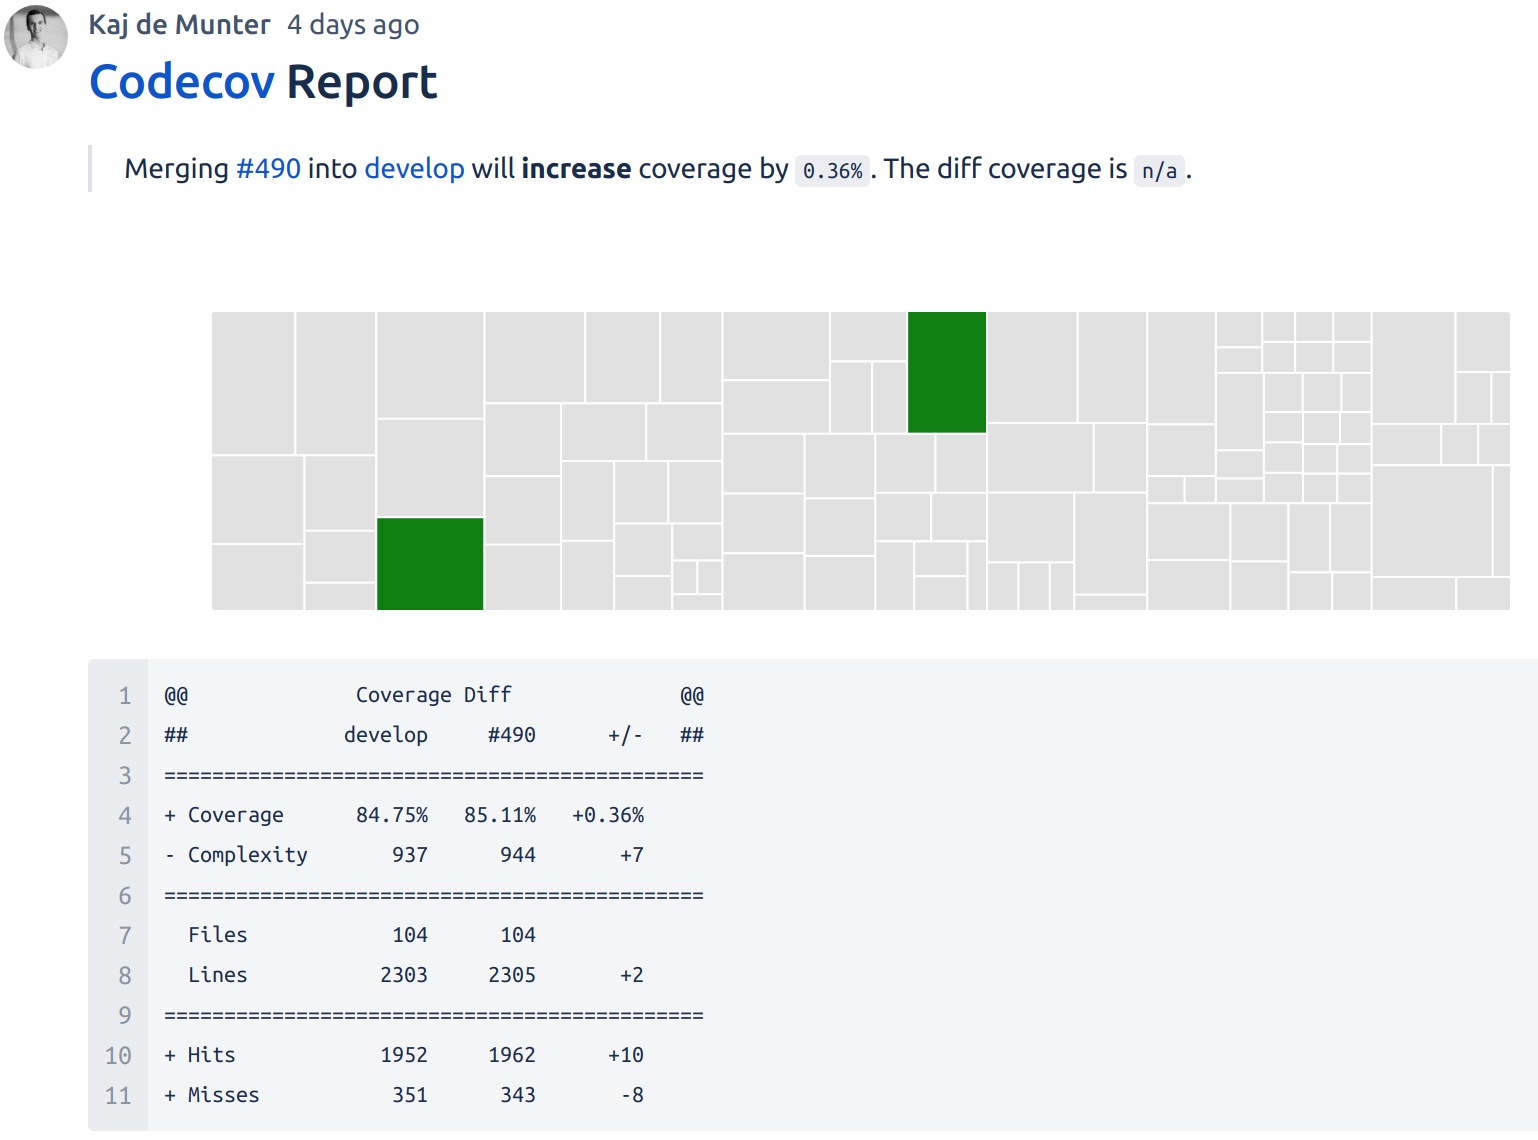
\includegraphics[width=13cm]{Figures/coverage}
	\decoRule
	\caption[Codecov bot]{Codecov bot reactie op een Pull-Request}
	\label{fig:coverage}
\end{figure}

Verder is er veel rekening gehouden met de beveiliging van de oplossing. Traefik draait niet als root in de container en de Docker Socket is beveiligd via TLS. Verder is OPA geïmplementeerd om beveiliging te waarborgen door middel van het limiteren van users die Docker commando's kunnen gebruiken. Ook is er een opzet gemaakt dat policies build-time kan evalueren zodat kwaliteit afgedwongen kan worden vóórdat het wordt gedeployed. Deze requirement is behaald.

\section{Monitoren van performance}

De implementatie van Grafana betekent dat er data uit allerlei verschillende databases gevisualiseerd kan worden. In dit onderzoek is als eerst besloten dat Prometheus een goede tool is om metrics te verzamelen. Uiteindelijk is geconcludeerd dat dit geen goede optie is. Daarom is de optie van monitoring vrijgesteld, maar er wordt nog niks daadwerkelijk gemonitord. Deze requirement is niet volledig behaald, daarom is er een aanbeveling gemaakt.

\section{Kwaliteitsstandaarden}
Door het monitoren van performance is de factor Telementry van de 15-Factor App verbeterd. De factor One Codebase, One application is niet verbeterd tijdens dit onderzoek, maar door middel van een generieke ansible infrastructuur kan deze verbeterd worden. Testbaarheid van ISO 25010 is verbeterd door het toevoegen van Codecov. 

Schalen in de context van horizontaal schalen is ook niet geïmplementeerd, maar door Feature-environments is wel bewezen dat de website schaalbaar is. Ook is advies uitgebracht over de methode van schalen door middel van de container orchestration tool Docker Swarm.

\section{Conclusie}

Must-requirements:
\begin{itemize}
	\item De oplossing moet méér dan twee unieke instanties van de website naast elkaar kunnen draaien.
    \begin{itemize}
        \item Behaald.
    \end{itemize}

	\item De oplossing moet moet unieke instanties van de website automatisch kunnen aanmaken.
    \begin{itemize}
        \item Behaald tot op zekere hoogte, de instanties kunnen nog niet automatisch worden verwijderd. Hier is een aanbeveling over gemaakt.
    \end{itemize}

	\item De oplossing moet een methode bevatten om kwaliteit van nieuwe toevoegingen aan de infrastructuur automatisch te waarborgen.
    \begin{itemize}
        \item Behaald. Er is een aanbeveling gemaakt om hier verder op in te gaan.
    \end{itemize}

	\item Minimaal één monitoring tool voor het monitoren van performance.
    \begin{itemize}
        \item Niet volledig behaald. Grafana is geïmplementeerd om data te visualiseren, maar er is nog geen data. 
    \end{itemize}

	\item De oplossing moet voldoen aan één of meerdere kwaliteitsstandaarden.
    \begin{itemize}
        \item Behaald, maar er zijn nog verbeteringen. Hier is een aanbeveling over gemaakt.
    \end{itemize}
\end{itemize}

Over de Should, Could en Won't requirements zijn aanbevelingen gemaakt in hoofdstuk \ref{Chapter8}.
